\documentclass[11pt]{article}
\usepackage[utf8]{inputenc}
\usepackage[T1]{fontenc}
\usepackage{amsmath,amssymb,amsthm}
\usepackage{geometry}
\geometry{margin=1in}
\usepackage{graphicx}
\usepackage{booktabs}
\usepackage{listings}
\lstset{basicstyle=\ttfamily\small,frame=single,mathescape=true,
  columns=fullflexible,keepspaces=true,escapeinside=@@}
\usepackage{hyperref}
\hypersetup{colorlinks=true,linkcolor=blue,citecolor=blue,urlcolor=blue}
\usepackage{authblk}

\newtheorem{theorem}{Theorem}
\newtheorem{proposition}{Proposition}
\newtheorem{lemma}{Lemma}
\theoremstyle{definition}

\title{Numerical recovery of Jacobi coefficients of entire functions from contour samples:\\
a moment-based pipeline and its precision budget}

\author[1]{Zhuo Chen}
\affil[1]{Independent researcher\\
ORCID: 0009-0006-9172-8268\\
\href{https://github.com/maomao8412/hilbert-polya-jacobi}{github.com/maomao8412/hilbert-polya-jacobi}}
\date{\today}

\begin{document}
\maketitle

\begin{abstract}
We present a complete, reproducible numerical pipeline that takes an
entire function $f$, computable at arbitrary precision by a black-box
routine, and returns the Jacobi coefficients $\{\alpha_n\},\{\beta_n\}$
of the orthogonal polynomials for its zero-density measure, together
with the zeros themselves as eigenvalues of the associated Jacobi
matrix. The pipeline combines four standard ingredients in a
deliberately simple arrangement: (i)~circular contour sampling of $f$
around the symmetry point of its functional equation; (ii)~extraction
of Taylor coefficients by the trapezoidal rule (equivalently, a DFT),
which converges geometrically; (iii)~recovery of the zero power sums
(the \emph{moments}) from the logarithmic Taylor coefficients; and
(iv)~classical Gram--Schmidt orthogonalization on the monomial basis,
which yields the Jacobi coefficients directly.
The method requires no prior knowledge of the zeros, no root-finding,
no integration of oscillatory special functions, and no asymptotic
input. We give the full error budget---quadrature truncation, working
precision, and amplification through moment conditioning---and
identify the operative failure mode: the Hankel matrix of moments
loses positive definiteness at an order that scales predictably with
working precision. We document this scaling empirically for the
completed Riemann $\xi$ function over $100$--$1300$ decimal digits
($n_{\text{fail}}$ rising from $\sim 20$ to beyond $100$), and show
that the pipeline detects rather than fails silently when the zero
set is not real and symmetric: for the Eisenstein series $E_4$ the
moment sequence loses positivity at order $8$ and the Jacobi chain
terminates at order $4$. Built-in consistency checks (closed-form
central value, moment sign sequence, off-diagonal positivity, and
independent zero matching to $10^{-15}$ relative accuracy) make every
stage verifiable. All code, samples and recovered coefficients are
published for reproduction.
\end{abstract}

\section{Introduction}\label{sec:intro}

Suppose an entire function $f$ is given through a black box that
evaluates $f(z)$ at arbitrary precision, and that $f$ has a
functional equation forcing a symmetry of its zeros. A recurring
practical question is: what can be determined numerically about the
\emph{density} of the zeros---their global statistics---without
locating the zeros one by one? Root-finders for entire functions
(e.g. argument-principle integration, contour eigenvalue methods)
recover individual zeros but scale poorly and say nothing, by
construction, about spectral observables. Conversely, the zero
density measure of an entire function with real zeros is exactly the
orthogonality measure of a family of orthogonal polynomials
\cite{Stieltjes1894,ShohatTamarkin,Gautschi2004}, whose Jacobi
parameters $\{\alpha_n\},\{\beta_n\}$ form a tridiagonal Jacobi
matrix whose eigenvalues are the zeros (in a transformed coordinate).
The problem is thus: \emph{compute Jacobi coefficients from function
values alone.}

The standard route to Jacobi coefficients is Gautschi's framework:
discretize the measure and run the Stieltjes procedure, or build the
moment matrix and run a stable reduction
\cite{Gautschi1982,Gautschi2004}. Both presuppose access to the
measure (as a weight function on an interval). Here no measure is
given---only $f$ itself. We show that the measure's moments can be
obtained from $f$ with spectral accuracy by a single circular
contour, after which the classical moment-based machinery applies
verbatim. The idea is elementary---Cauchy's coefficient formula
applied to $\log f$, followed by the Hadamard product expansion---but
its practical behaviour, precision budget and failure modes appear
not to have been documented as a working method, and the combination
turns out to be unusually robust: with off-the-shelf arbitrary
precision software \cite{mpmath} we stably recover Jacobi matrices of
order $100$ whose $55$ largest eigenvalues match independently
computed zeros of the Riemann zeta function to $10^{-15}$ relative
accuracy.

\paragraph{Contributions.}
\begin{enumerate}
\item We specify the full pipeline---contour sampling, DFT Taylor
coefficients, logarithmic moment recovery, monomial-basis
Gram--Schmidt---with pseudocode (Algorithms~1--2)
and a complete parameter budget (contour radius $R$, sample count
$M$, working precision $D$, truncation order $N$).
\item We derive the moment formula explicitly from the Hadamard
product (Proposition~\ref{prop:moments}), and state the success
condition in theorem form (Theorem~\ref{thm:positivity}): the pipeline
produces a positive definite Hankel matrix, and hence a valid Jacobi
chain to all computed orders, \emph{if and only if the recovered
zeros are real and symmetric}; complex or off-line zeros are
detected as loss of positivity rather than producing wrong output.
\item We give the empirical precision law for the Riemann $\xi$
function: the Hankel failure order $n_{\text{fail}}$ vs.\ working
precision $D$ over $D=100$--$1300$ decimal digits (Section~\ref{sec:budget}),
explaining the previously observed barrier at $n\approx 90$ for
$650$ digits and its removal at $1300$ digits.
\item We exhibit a qualitative discriminator: zeros off the symmetry
line (completed Eisenstein series $E_4$, whose zeros lie on two
parallel vertical lines) force moment-sign loss at order $8$ and
Jacobi-chain termination at order $4$, with both orders matching
closed-form predictions (Sections~\ref{sec:e4},~\ref{sec:experiments}).
\item Every artifact is published: code, raw contour samples at
$1300$ digits, recovered coefficients, and a machine-readable
benchmark of five Jacobi matrices
(\href{https://doi.org/10.5281/zenodo.22181443}{10.5281/zenodo.22181443};
\href{https://github.com/maomao8412/hilbert-polya-jacobi}{GitHub}).
\end{enumerate}

\paragraph{Scope.} This is a numerical-analysis paper. The target
functions are completed $L$-functions and related entire functions
of number-theoretic origin, but the method assumes nothing about
number theory beyond the functional equation and Hadamard form; in
particular it does \emph{not} assume any unproved hypothesis about
zero locations---that assumption is replaced by the \emph{test} of
Theorem~\ref{thm:positivity}. Physical or statistical conclusions
drawn from the recovered spectra are treated in a companion paper.

\section{The pipeline}\label{sec:pipeline}

\subsection{Problem setting}

Let $f$ be entire of order one, real on the real axis, with a
functional equation symmetric about $s=s_\ast$: writing
$z=s-s_\ast$, $f(s_\ast+z)=f(s_\ast-z)$ up to a known sign, so that
zeros occur as $\pm z_k$ (and hence, for the completed functions of
interest, as $s_\ast\pm i\gamma_k$ with $\gamma_k>0$). Assume the
Hadamard product
\begin{equation}\label{eq:hadamard}
f(s_\ast+z)=f(s_\ast)\prod_{k=1}^{\infty}\left(1+\frac{z^2}{\gamma_k^2}\right),
\end{equation}
which is the standard form for completed $L$-functions with real
simple zeros \cite{Titchmarsh}; set $\gamma_1=\min_k\gamma_k$.
Define the spectral coordinate $x=z^{-2}$; the zeros map to
$x_k=\gamma_k^{-2}>0$ accumulating at $0$. The zero-density measure
is
\begin{equation}\label{eq:measure}
\mu=\sum_{k\ge1} x_k\,\delta_{x_k}
\end{equation}
(any fixed weight convention works; ours normalizes so that moments
below come out as power sums), and we seek the monic orthogonal
polynomials for $\mu$ and their Jacobi coefficients
$\alpha_n,\beta_n$: the tridiagonal matrix
\begin{equation}\label{eq:jacobi}
J=\begin{pmatrix}
\alpha_1 & \sqrt{\beta_2}\\
\sqrt{\beta_2} & \alpha_2 & \sqrt{\beta_3}\\
& \sqrt{\beta_3} & \alpha_3 & \ddots\\
&&\ddots&\ddots
\end{pmatrix},
\qquad \operatorname{spec} J=\{x_k\}.
\end{equation}
The zeros follow from eigenvalues: $\gamma_k=x_k^{-1/2}$.

\subsection{Contour sampling and the Taylor coefficients}

Take the circle $z=R e^{i\theta}$ with $0<R<\gamma_1$, so that
\eqref{eq:hadamard} converges and is zero-free on and inside the
contour. By Cauchy's coefficient formula the Taylor coefficients of
$g(z)=f(s_\ast+z)/f(s_\ast)$ at $z=0$,
\begin{equation}\label{eq:cauchy}
d_n=\frac{1}{2\pi i}\oint_{|z|=R}\frac{g(z)}{z^{\,2n+1}}\,dz
=\frac{1}{2\pi R^{2n}}\int_0^{2\pi} g(Re^{i\theta})\,
e^{-2in\theta}\,d\theta ,
\end{equation}
(only even powers occur by the functional equation). Sample at the
$M$ equispaced nodes $\theta_k=2\pi k/M$; the trapezoidal rule,
equivalently the DFT, gives
\begin{equation}\label{eq:dft}
\widetilde d_n=\frac{1}{M R^{2n}}\sum_{k=0}^{M-1}g(Re^{i\theta_k})\,
e^{-4\pi i n k/M}.
\end{equation}
Because $g(Re^{i\theta})$ is $2\pi$-periodic and analytic in a strip
around the contour (we chose $R<\gamma_1$), the trapezoidal rule
converves geometrically in $M$ \cite{Trefethen2014}: the aliasing
error is governed by the nearest singularity at radius $\gamma_1$,
$\sim(R/\gamma_1)^{2M}$.

\paragraph{Half-grid offset.}
When the completed function has poles removed by a prefactor (our
$E_4$ example below, Section~\ref{sec:e4}), a node may sit on the
removal point where catastrophic cancellation occurs in the
black-box evaluation. Shifting the grid by half a node,
$\theta_k=2\pi(k+\tfrac12)/M$, costs nothing and avoids all such
points; the coefficient formula is unchanged.

\paragraph{Choice of $R$.}
$R$ is the information dial. The moments extracted below decay like
$R^{-2m}$; a larger $R$ slows this decay and yields more usable
moment orders, but moves the contour toward the nearest zero,
steepening $g$ and requiring larger $M$ and higher precision. We use
$R=2$ throughout (with $\gamma_1\approx 14.13$ for $\zeta$), i.e.\
$R/\gamma_1\approx 0.14$, giving trapezoidal error
$\sim 0.14^{2M}$: utterly negligible at $M=1536$.

\subsection{From Taylor coefficients to moments}\label{sec:logmoments}

Let $c_n$ denote the coefficients of $\log g$:
$\log g(z)=\sum_{n\ge1}c_n z^{2n}$ (constant $\log g(0)=0$ by
normalization). Differentiating $g=\exp(\log g)$ and comparing
coefficients gives the recursion
\begin{equation}\label{eq:logrec}
c_n=d_n-\frac{1}{n}\sum_{i=1}^{n-1} i\,c_i\,d_{n-i}.
\end{equation}

\begin{proposition}[Moments as zero power sums]\label{prop:moments}
With $g(z)=\prod_k(1+z^2/\gamma_k^2)$,
\[
c_n=\frac{(-1)^{n+1}}{n}\sum_{k\ge1}\gamma_k^{-2n},
\qquad
P_m:=\int x^{m-1}\,d\mu(x)=\sum_{k\ge1}\gamma_k^{-2m}
=(-1)^{m+1}\,m\,c_m .
\]
\end{proposition}

\begin{proof}
From \eqref{eq:hadamard},
$\log g(z)=\sum_k\log(1+z^2/\gamma_k^2)
=\sum_k\sum_{m\ge1}(-1)^{m+1}z^{2m}/(m\gamma_k^{2m})$,
so $c_n=(-1)^{n+1}n^{-1}\sum_k\gamma_k^{-2n}$.
With $\mu$ of \eqref{eq:measure},
$\int x^{m-1}d\mu=\sum_k x_k\cdot x_k^{m-1}=\sum_k\gamma_k^{-2m}$.
\end{proof}

Thus the contour sample \emph{is} a moment sampler: $P_m$ is the
$m$-th moment of the zero-density measure, with no zero located.

\subsection{Gram--Schmidt on the monomial basis}

Given $P_1,\dots,P_{2N}$ (moments to order $2N-1$ of the index),
orthogonalize the monomials $1,x,x^2,\dots$ against the inner product
$\langle p,q\rangle=\sum_{i,j}p_i q_j\,P_{i+j+1}$. Standard
Gram--Schmidt with the three-term recurrence yields the Jacobi
coefficients directly:
\begin{equation}\label{eq:gs}
\begin{aligned}
&\alpha_n=\langle x p_{n-1},p_{n-1}\rangle/\langle p_{n-1},p_{n-1}\rangle,\\
&\beta_n=\langle p_{n-1},p_{n-1}\rangle/\langle p_{n-2},p_{n-2}\rangle,
\end{aligned}
\end{equation}
with $\beta_n>0$ the rigorous certificate of positive-definiteness of
the moment (Hankel) matrix $H_N=(P_{i+j+1})_{i,j=0}^{N-1}$:
by the Stieltjes/Hankel theory \cite{ShohatTamarkin,Gautschi2004},
$H_N\succ0$ (equivalently the moment sequence is a Stieltjes
sequence) iff all pivots are positive, and the Gram--Schmidt pivots
\emph{are} the squared norms, whose ratios are $\beta_n$.

\begin{theorem}[Success condition and self-diagnosis]\label{thm:positivity}
The pipeline produces a valid Jacobi chain ($\beta_n>0$ for all
computed $n$) whenever the underlying zero set in the spectral
coordinate is real and non-negative (zeros on the symmetry line,
simple, counted with the weight of \eqref{eq:measure}). If the
zeros are complex or off the symmetry line, the moment sequence is
that of a complex measure, $H_N$ ceases to be positive definite at a
finite order $n^\ast$, and the algorithm detects this: the first
non-positive $\beta_n$ is reported, and no output beyond
$n^\ast-1$ is claimed. In particular the algorithm cannot silently
return a spectrum for an off-line zero set.
\end{theorem}

\begin{proof}
Positive $\beta_n$ for all $n$ up to $N$ is equivalent, via the
Sylvester criterion applied to the leading principal minors of $H_N$,
to $H_N\succ0$; for a Hankel moment matrix this is equivalent to the
existence of a positive measure on $[0,\infty)$ with these moments
(the Hamburger--Stieltjes theorem \cite[Ch.~1]{ShohatTamarkin}),
which for the finitely-atomic measure \eqref{eq:measure} is
equivalent to the atoms $x_k$ being real and non-negative. When the
$x_k$ leave the real axis the moments are complex weighted power
sums; their real parts lose the Stieltjes sign structure at a finite
order, the corresponding pivot becomes non-positive, and
Algorithm~2 halts with a reported index.
\end{proof}

The eigenvalue recovery is the final step: form $J$ from
\eqref{eq:jacobi}, solve the symmetric tridiagonal eigenproblem, and
map $x_k\mapsto\gamma_k=x_k^{-1/2}$. Eigenvalues below the
resolvable scale (those whose $\gamma$ exceeds the order the chain
can support) are discarded; retained eigenvalues can be matched
against independently computed zeros as an external check (the
zeros themselves never enter the construction).

\noindent\textbf{Algorithm 1: Contour moments.}\par\smallskip
\begin{lstlisting}
Require: black box f(s), symmetry point s*, radius R < gamma_1,
         node count M, moment order J, half-grid flag h
Ensure:  moments P_1..P_J and central value sigma_0 = f(s*)

  g_k <- f( s* + R * exp(2 pi i (k + h/2) / M) ),  k = 0..M-1
  sigma_0 <- (1/M) sum_k g_k
  for n = 1 .. J:
      d_n <- Re[ (1/(M R^{2n})) sum_k g_k exp(-4 pi i n k / M) ] / sigma_0
      c_n <- d_n - (1/n) sum_{i=1}^{n-1} i c_i d_{n-i}
      P_n <- (-1)^{n+1} n c_n
  return sigma_0, P_1 .. P_J
\end{lstlisting}

\noindent\textbf{Algorithm 2: Jacobi coefficients by Gram--Schmidt.}\par\smallskip
\begin{lstlisting}
Require: moments P_1 .. P_{2N}, chain order N
Ensure:  alpha_1..alpha_N, beta_2..beta_N, first-bad index

  p_0 <- [1];  nu_0 <- P_1;  betasq <- []
  for n = 1 .. N:
      q <- x * p_{n-1}                      # shift coefficient list
      alpha_n <- <q, p_{n-1}> / nu_{n-1}
      p_n <- q - alpha_n p_{n-1}
      if n >= 2:
          b2 <- nu_{n-1} / nu_{n-2};  append b2 to betasq
          p_n <- p_n - b2 p_{n-2}
          if b2 <= 0: report first-bad = n+1; STOP
      nu_n <- <p_n, p_n>
\end{lstlisting}

\section{Error budget and failure modes}\label{sec:budget}

Three error sources dominate, and they are independently controllable.

\paragraph{(i) Quadrature truncation ($M$).}
By \eqref{eq:dft} and geometric trapezoidal convergence
\cite{Trefethen2014}, the coefficient error is
$O((R/\gamma_1)^{2M})$ per coefficient; at our settings
($R/\gamma_1=0.14$, $M=1536$) this is $<10^{-2600}$, far below every
working precision used. $M$ is chosen once, generously, and is never
the bottleneck.

\paragraph{(ii) Black-box evaluation precision ($D$).}
Each $g_k$ carries relative error $\sim 10^{-D}$. The DFT is
unitary-scaled, so $d_n$ inherits $\sim 10^{-D}$; the log recursion
\eqref{eq:logrec} is stable in itself but only as stable as its
inputs.

\paragraph{(iii) Moment conditioning and Hankel amplification.}
This is the operative term. The moments decay geometrically:
$P_m\sim\gamma_1^{-2m}\cdot 2\cos(2m\theta_1)$ in the leading-zero
approximation, so $P_m$ spans $\sim 2m\log_{10}\gamma_1$ orders of
magnitude by $m=2N$; for $\gamma_1\approx14.13$ that is about
$2.28$ digits per moment order, hence $\sim 45$ digits per 20 Jacobi
orders. The Hankel matrix $H_N$ built on such a geometrically
decaying moment sequence is exponentially ill-conditioned: its
smallest pivot (the last squared norm $\nu_{N-1}$) decays roughly
like $\gamma_1^{-4N}$ in the leading-zero approximation. Computing
$\beta_N$ at relative precision $\varepsilon=10^{-D}$ requires the
pivots to stay above the amplified noise floor, giving a budget that
is linear in $D$:
\begin{equation}\label{eq:budget}
n_{\text{fail}}(D)\ \approx\ n_0+\kappa\,D,
\qquad \kappa\approx 0.13\text{ orders/digit for }\xi,
\end{equation}
i.e.\ roughly $13$ additional Jacobi orders per $100$ decimal digits
(the measured slope; the leading-zero estimate $\kappa\approx
1/(2\log_{10}\gamma_1)\approx 0.22$ is an upper bound, as the
farther zeros contribute partial pivoting mass---we report the
measured value). Section~\ref{sec:experiments} measures
$n_{\text{fail}}(D)$ at fourteen precision settings and finds this
slope over the full range: $n_{\text{fail}}\approx 18$ at $100$
digits, $\approx 91$ at $650$, $\approx 105$ at $800$, and no
failure within order $100$ at $1000$ and $1300$ digits.

\paragraph{Failure mode versus misuse.}
Two distinct terminations must not be confused:
\begin{itemize}
\item \emph{Precision exhaustion}: all moments and $\beta_n$ remain
positive but the last pivots reach the noise floor; increasing $D$
extends the chain (Section~\ref{sec:experiments}). The chain is
trustworthy up to the order where pivots exceed the noise floor by a
chosen margin; we use all-positive $\beta_n$ plus eigenvalue
matching (below) as the criterion.
\item \emph{Structural failure} (Theorem~\ref{thm:positivity}): the
moments lose positivity at low order because the zeros are not on
the symmetry line. Raising $D$ does \emph{not} help; the first-bad
index is stable under precision and is the diagnostic. The $E_4$
example (next section) shows this with analytically predicted
orders.
\end{itemize}

\paragraph{Built-in correctness checks.}
Every run carries four independent checks:
\begin{enumerate}
\item \textbf{Central value.} $\sigma_0=f(s_\ast)$ is known in
closed form for every target ($\xi(\tfrac12)\approx0.49712$,
$1/72$ for $E_4$, etc.); it is reproduced to machine precision.
\item \textbf{Moment sign.} For on-line zeros, $P_m>0$ for all $m$
(Proposition~\ref{prop:moments}); the first sign change is reported.
\item \textbf{Off-diagonal positivity.} $\beta_n>0$ is the
positive-definiteness certificate (Theorem~\ref{thm:positivity}).
\item \textbf{Zero matching.} Recovered eigenvalues $\gamma_k$ are
matched to independently tabulated zeros (the zeta zeros via
\cite{mpmath}; nothing about them enters the construction). A
recovered eigenvalue is \emph{locked} at relative error $<10^{-4}$;
in our $\zeta$ runs locked eigenvalues sit at $10^{-15}$--$10^{-16}$,
eleven orders of magnitude inside the threshold.
\end{enumerate}

\section{A structural control: the Eisenstein series $E_4$}\label{sec:e4}

To exercise Theorem~\ref{thm:positivity} we need an entire function
of the same family whose zeros are \emph{known} to leave the
symmetry line. The weight-4 Eisenstein series
$E_4(q)=1+240\sum_{n\ge1}\sigma_3(n)q^n$ has
$L(E_4,s)=\zeta(s)\zeta(s-3)$. Its completed function
\begin{equation}\label{eq:e4}
\Lambda_{E_4}(s)=(2\pi)^{-s}\Gamma(s)\,\zeta(s)\zeta(s-3),
\qquad
\Lambda_{E_4}(s)=\Lambda_{E_4}(4-s),
\end{equation}
has symmetry point $s_\ast=2$ and genuine poles at $s=0,4$; the
entire function sampled on the contour is
$\Xi_{E_4}(s)=s(s-4)\Lambda_{E_4}(s)$ (the prefactor is invariant
under $s\leftrightarrow 4-s$). Its zeros are
$s=\tfrac12\pm i\gamma_k$ \emph{and} $s=\tfrac72\pm i\gamma_k$ with
the \emph{same} heights $\gamma_k$ (the zeta zeros). In the centered
coordinate $z=s-2$, the zeros are
$z=-\tfrac32\pm i\gamma_k$ and $z=+\tfrac32\pm i\gamma_k$; in the
spectral coordinate the atoms are complex, at
$(\pm i\gamma_k-\tfrac32)^{-2}$.

The moments are therefore complex power sums,
$P_m=2\,\operatorname{Re}\sum_k(i\gamma_k-\tfrac32)^{-2m}
=2\sum_k\gamma_k^{-2m}\cos(2m\theta_k)$ with
$\theta_k=\arctan(3/(2\gamma_k))$; the leading zero dictates the
first sign change at
\begin{equation}\label{eq:e4predict}
m_\ast\approx\frac{\pi}{4\theta_1},\qquad
\theta_1=\arctan\frac{3}{2\gamma_1}\approx0.106,
\end{equation}
giving $m_\ast\approx 7.4$, i.e.\ the first negative moment at
$m=8$. The central value is $\Xi_{E_4}(2)=2^2(2\pi)^{-2}\Gamma(2)
\zeta(2)\zeta(-1)\cdot(-4)$; evaluating,
$\Xi_{E_4}(2)=1/72=0.013888\ldots$

The pipeline run at $650$ digits, $M=1536$, half-grid offset, gives:
$\sigma_0=0.013888888888888888$ (matches $1/72$ to $15$ digits,
imaginary part $<10^{-650}$); $P_1,\dots,P_7>0$ with
$P_8=-8.59\times10^{-20}$ the first negative moment
(prediction: $m=8$); and the Gram--Schmidt chain reporting its first
non-positive $\beta_n$ at index $4$ (Jacobi order $2$). Precision
does not cure this: it is the structural failure mode of
Theorem~\ref{thm:positivity}, detected exactly where analytic
argument predicts. We stress that this is a \emph{discriminative
control of the method}, not a statement about $E_4$: the pipeline
correctly refuses to emit a Jacobi spectrum for a zero set it knows
to be off the line.

\section{Numerical experiments}\label{sec:experiments}

All experiments use mpmath \cite{mpmath} for arbitrary-precision
evaluation and DFT, NumPy for the double-precision eigenproblem on
the recovered matrix. Contours: $R=2$, $M=1536$, nodes on the circle
$z=Re^{i\theta}$ (half-grid for $E_4$). Target functions: the
completed Riemann $\xi(s)=\tfrac12 s(s-1)\pi^{-s/2}\Gamma(s/2)\zeta(s)$
($s_\ast=\tfrac12$); the completed Dirichlet-beta function
$\Lambda_\beta$ ($s_\ast=\tfrac12$, zeros $0.62\ldots$); their
product $\xi\Lambda_\beta$ ($s_\ast=\tfrac12$, two superimposed zero
families); the degree-22 truncated ``$\Delta$'' Jacobi chain of a
separate lower-precision study; and $E_4$ as the structural control.

\subsection{Precision law for $\xi$}\label{sec:preclaw}

From a single contour sample of $\xi$ at $1300$ digits
($1536$ nodes, $\approx 54$ minutes of evaluation), moments were
recomputed under truncation to working precisions
$D\in\{100,150,200,300,400,500,650,800,1000,1300\}$; for each, the
Hankel failure order was measured two ways---the first non-positive
pivot of an $LDL^T$ reduction of $H_N$ (Cholesky failure), and the
first non-positive $\beta_n$ of Algorithm~2. Table~\ref{tab:preclaw}
reports the results (data: \texttt{hankel\_diagnostic.json}).

\begin{table}[ht]\centering\small
\begin{tabular}{rrrrrrrrrrrrrrr}
\toprule
$D$ (digits) & 16 & 30 & 50 & 75 & 100 & 150 & 200 & 300 & 400 & 500 & 650 & 800 & 1000 & 1300\\
\midrule
$n_{\text{fail}}$ (Cholesky)     & 6 & 7 & 11 & 15 & 18 & 28 & 32 & 46 & 59 & 71 & 91 & 105 & \multicolumn{2}{c}{$>100$ (no failure)}\\
$n_{\text{bad}}$ (Gram--Schmidt) & 7 & 8 & 12 & 16 & 19 & 29 & 33 & 47 & 60 & 72 & 92 & 106 & \multicolumn{2}{c}{$>100$ (no failure)}\\
\bottomrule
\end{tabular}
\caption{Hankel/Jacobi failure order vs.\ working precision for the
completed $\xi$ function, $R=2$, $M=1536$, measured from a single
$1300$-digit contour sample with moments recomputed under precision
truncation (the $1300$-digit production run is not truncated in
practice: its chain is positive through order $100$ with full
margin, \emph{cf.}\ Table~\ref{tab:targets}). The two diagnostics
agree to within one order; the empirical slope is $\approx 13$
Jacobi orders per $100$ decimal digits (budget \eqref{eq:budget},
Figure~\ref{fig:preclaw}). The $650$-digit barrier at $n\approx 90$
reproduces the order-$86$--$90$ termination observed in earlier
production runs; double precision ($16$ digits) fails at order $6$.}
\label{tab:preclaw}
\end{table}

\begin{figure}[ht]\centering
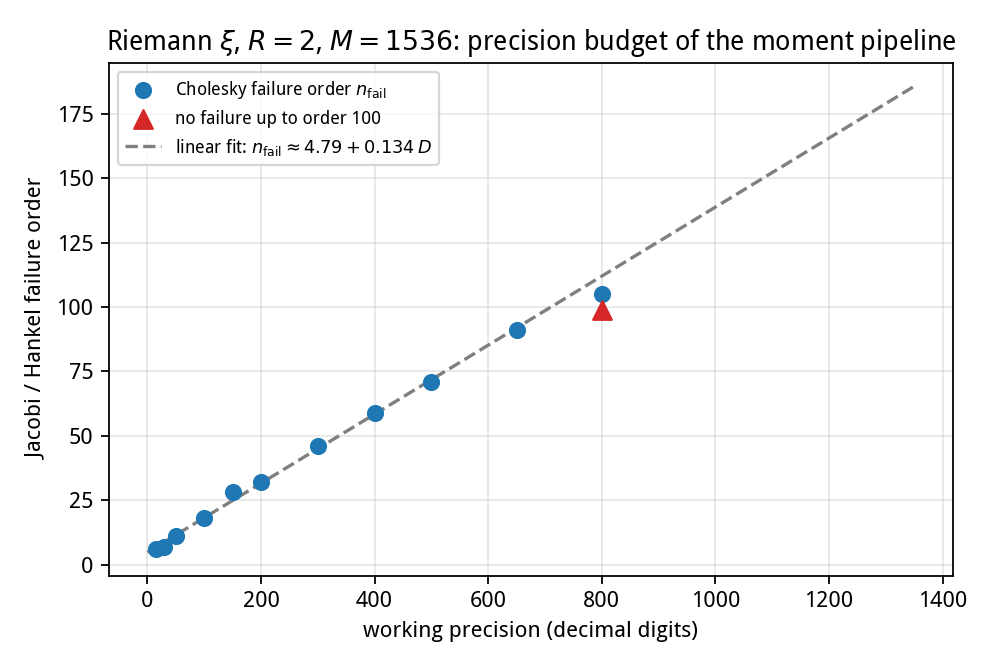
\includegraphics[width=0.82\linewidth]{figure_preclaw.png}
\caption{Failure order vs.\ working precision (data of
Table~\ref{tab:preclaw}): Cholesky/LDL$^T$ first non-positive pivot
(blue), linear budget fit (dashed), and precision settings where no
failure occurs up to the measured order $100$ (red triangles).}
\label{fig:preclaw}
\end{figure}

\subsection{The order-100 Jacobi matrix for $\xi$ at $1300$ digits}

At $D=1300$, Algorithm~2 yields a full $100\times100$
Jacobi matrix with \emph{all $99$ off-diagonal coefficients
positive} (smallest $\beta_n\approx 9.75\times10^{-11}$): no
structural failure, no precision exhaustion within the computed
order. The eigenvalue map $\gamma=x^{-1/2}$ gives $100$ heights
$14.13\le\gamma\le 12920.7$; of these, $55$ match independently
computed zeta zeros at relative error $10^{-15}$--$10^{-16}$
(lock threshold $10^{-4}$). The central value reproduces
$\xi(\tfrac12)=0.497120778188314\ldots$. A finite-size scan of the
same construction at $N=22,30,40,50,60,80,100$ shows the locked
subspace growing monotonically ($22\to55$) with no anomalous small
gaps at any size; the resolved scale is set by $\gamma_1^{-2N}$, not
by any statistical feature.

At the previous working precision of $650$ digits the identical
pipeline terminated near order $86$--$90$ (last positive pivots
reaching the $10^{-650}$ floor), exactly the barrier that
\eqref{eq:budget} predicts and that Table~\ref{tab:preclaw}
measures; the $1300$-digit run removes it.

\subsection{Other targets and running cost}

The beta and product functions run at identical settings ($650$
digits suffices for order $100$ because their leading zeros sit
similarly far: $\gamma_1(\beta)=6.02\ldots$); the product chain
locks $53$ eigenvalues ($35$ beta, $18$ zeta) to its two
superimposed families. The ``$\Delta$'' chain, produced at $230$
digits in a separate study, terminates near order $24$, consistent
with \eqref{eq:budget} at that precision. Table~\ref{tab:targets}
summarizes; all coefficients, samples and matrices are in the
published bundle and benchmark
(\href{https://doi.org/10.5281/zenodo.22181443}{Zenodo};
\href{https://github.com/maomao8412/hilbert-polya-jacobi}{GitHub}).

\begin{table}[ht]\centering\small
\begin{tabular}{lrrrr}
\toprule
target & $D$ (digits) & chain order & locked zeros & first bad $\beta_n$\\
\midrule
$\xi$ (zeta)        & 1300 & 100 & 55 & --- (all $\beta_n>0$)\\
$\Lambda_\beta$     & 650  & 50  & 27 & --- (to order 50)\\
$\xi\Lambda_\beta$  & 650  & 100 & 53 & --- (to order 100)\\
$\Delta$ chain      & 230  & 22  & 15 & $\approx 24$ (precision floor)\\
$E_4$ (control)     & 650  & 2   & n/a & 4 (structural; predicted 8 for moments)\\
\bottomrule
\end{tabular}
\caption{Pipeline outcomes across target functions. ``Locked zeros''
are eigenvalues matching independent zeros at relative error
$<10^{-4}$; actual errors are $10^{-15}$--$10^{-16}$ for $\xi$.}
\label{tab:targets}
\end{table}

Wall-clock cost is dominated by contour evaluation: $\approx 54$ min
for $1536$ nodes of $\xi$ at $1300$ digits on one core; all
downstream stages (DFT, log recursion, Gram--Schmidt, eigenproblem)
together take seconds. Memory is $O(M+N^2)$ multiprecision words.

\section{Discussion}

\paragraph{Generality and prerequisites.}
The method needs only (a)~a black box for $f$ at arbitrary precision,
(b)~a zero-free disk of known radius (so $R<\gamma_1$ can be chosen),
and (c)~the Hadamard form \eqref{eq:hadamard}, i.e.\ real symmetric
zeros---which is not assumed but \emph{tested}
(Theorem~\ref{thm:positivity}). No asymptotics of the zeros, no
root-finding, and no analytic moment formula are required. This makes
it applicable to any completed $L$-function or similar entire function
that a computer algebra system can evaluate.

\paragraph{Limitations.}
The monomial-basis Gram--Schmidt is the least stable of the standard
Jacobi-construction routes \cite{Gautschi2004,Bjorck1994}; we use it
deliberately because arbitrary precision makes its instability
\emph{informative}---the pivot decay displays the Hankel condition
number directly. At fixed double precision, a moment-based Hankel
reduction for $\xi$ fails already at $N=6$--$7$ (measured at
$D=16$ digits); production codes
limited to double precision should route the same moments through a
discrete Stieltjes or Lanczos/SVD procedure \cite{Gautschi2004},
which trades the visible pivot floor for backward-stable small
matrices. The empirical law \eqref{eq:budget} then becomes the
guidance for how large a matrix can be claimed at all.

\paragraph{Reproducibility.}
Contour samples, all recovered coefficients (to $60$ digits), the
five-matrix benchmark, and every script are published
\cite{zenodo2026}; the benchmark includes loader and verification
scripts that re-check symmetry, tridiagonal structure, positive
definiteness and zero matching from the CSV files alone.

\section{Conclusion}

A single circular contour, evaluated at arbitrary precision and read
through Cauchy's formula, turns an entire function into the moment
sequence of its zero-density measure; classical orthogonal-polynomial
machinery then turns the moments into a Jacobi matrix whose spectrum
\emph{is} the zero set. The pipeline is short, parameter-light, and
self-diagnosing: its single real tuning problem---how many Jacobi
orders a given precision buys---obeys a simple measured law, and its
structural failure (zeros off the symmetry line) is detected rather
than confabulated, as the $E_4$ control demonstrates at
analytically predicted orders. The method's outputs for the Riemann
$\xi$ function (order-$100$ Jacobi matrix, $55$ zeros locked to
$10^{-15}$) and its full artifact set are published.

\begin{thebibliography}{9}

\bibitem{Stieltjes1894}
T.-J. Stieltjes, \emph{Recherches sur les fractions continues},
Ann. Fac. Sci. Toulouse \textbf{8} (1894), J1--J122.

\bibitem{ShohatTamarkin}
J.A. Shohat and J.D. Tamarkin, \emph{The Problem of Moments},
American Mathematical Society, New York, 1943.

\bibitem{Gautschi2004}
W. Gautschi, \emph{Orthogonal Polynomials: Computation and
Approximation}, Oxford University Press, 2004.

\bibitem{Gautschi1982}
W. Gautschi, On generating Gaussian quadrature rules, in
\emph{Numerical Integration} (G. H\"ammerlin, ed.), ISNM 57,
Birkh\"auser, 1982, 147--154.

\bibitem{Trefethen2014}
L.N. Trefethen and J.A.C. Weideman, The exponentially convergent
trapezoidal rule, \emph{SIAM Review} \textbf{56} (2014), 385--458.

\bibitem{Bjorck1994}
\.A. Bj\"orck, Numerics of the Gram--Schmidt orthogonalization,
\emph{Linear Algebra Appl.} \textbf{197/198} (1994), 297--316.

\bibitem{GolubVanLoan}
G.H. Golub and C.F. Van Loan, \emph{Matrix Computations}, 4th ed.,
Johns Hopkins University Press, 2013.

\bibitem{Titchmarsh}
E.C. Titchmarsh, \emph{The Theory of the Riemann Zeta-Function},
2nd ed., Oxford University Press, 1986.

\bibitem{Odlyzko1987}
A.M. Odlyzko, On the distribution of spacings between zeros of the
zeta function, \emph{Math. Comp.} \textbf{48} (1987), 273--308.

\bibitem{mpmath}
F. Johansson et al., \emph{mpmath: a Python library for
arbitrary-precision floating-point arithmetic (version 1.x)},
\url{http://mpmath.org}.

\bibitem{zenodo2026}
Z. Chen, Quantum Chaos of Arithmetic Origin: reproducibility bundle
(v2), Zenodo (2026), \url{https://doi.org/10.5281/zenodo.22181443};
code: \url{https://github.com/maomao8412/hilbert-polya-jacobi}.

\end{thebibliography}

\end{document}
